% Fusionner l'IR et la CSG : note de chiffrage (rapport Sorbon, partie III, mesure 3)
% Compilation depuis fiscalite/ir_csg/ : pdflatex note-ir-csg.tex (deux passes)
% Figures nues : FIG_NU=1 python3 ir_csg/ir_csg.py ; FIG_NU=1 python3 ir_csg/optimal.py (depuis fiscalite/)
% Chiffres : ir_csg/sorties/{baremes,par_tranche,robustesse,optimal}.txt|csv
\documentclass[11pt,a4paper]{article}
% Préambule commun au brief et à la revue de littérature sur la taxe sur la valeur foncière.
% Même composition que le cours (cours/refaire-l-impot.tex) ; figures « nues » produites par
%   FIG_NU=1 python lvt/graphiques_lvt.py
\usepackage[T1]{fontenc}
\usepackage[utf8]{inputenc}
\usepackage{lmodern}
\usepackage[french]{babel}
\usepackage[a4paper,left=2.8cm,right=2.8cm,top=2.6cm,bottom=2.8cm]{geometry}
\usepackage{graphicx}
\usepackage[export]{adjustbox}
\usepackage{booktabs}
\usepackage{tabularx}
\usepackage{array}
\usepackage{xcolor}
\usepackage{titlesec}
\usepackage[labelfont=bf,labelsep=period,font=small,singlelinecheck=false,
            justification=raggedright,skip=6pt]{caption}
\usepackage{fancyhdr}
\usepackage{enumitem}
\usepackage{microtype}
\usepackage{textcomp}
\usepackage{amsmath}
\providecommand{\euro}{\texteuro}
\usepackage[hidelinks]{hyperref}

\definecolor{encre}{HTML}{1A1A19}
\definecolor{bleu}{HTML}{003399}
\definecolor{vert}{HTML}{1F7A4D}
\definecolor{ocre}{HTML}{C79100}
\definecolor{brique}{HTML}{993333}
\definecolor{filet}{HTML}{C8C6BE}

\titleformat{\section}{\normalfont\large\bfseries\color{bleu}}{\thesection.}{0.6em}{}
\titleformat{\subsection}{\normalfont\normalsize\bfseries\color{bleu}}{\thesubsection}{0.6em}{}
\titlespacing*{\section}{0pt}{2.4ex plus 1ex minus .2ex}{1.2ex plus .2ex}
\titlespacing*{\subsection}{0pt}{2ex plus 1ex minus .2ex}{0.8ex plus .2ex}

\pagestyle{fancy}
\fancyhf{}
\renewcommand{\headrulewidth}{0.4pt}
\fancyhead[R]{\small\thepage}

\setlength{\parindent}{0pt}
\setlength{\parskip}{0.62em}
\linespread{1.05}
\renewcommand{\arraystretch}{1.2}
\setlist{itemsep=2pt,topsep=2pt,parsep=0pt,leftmargin=1.4em}

\newenvironment{encadre}[1]
  {\par\medskip\noindent\begin{minipage}{\linewidth}%
   \color{encre}\setlength{\parskip}{0.5em}%
   \hrule height 0.8pt width \linewidth \vspace{6pt}%
   {\footnotesize\bfseries\color{vert}\MakeUppercase{#1}}\par\vspace{-2pt}%
   \small}
  {\par\vspace{4pt}\hrule height 0.4pt width \linewidth\end{minipage}\par\medskip}

\newcommand{\figbloc}[3]{%
  \begin{figure}[htbp]\centering
  \caption{#2}\label{#3}
  \includegraphics[max width=\linewidth,max height=0.40\textheight]{../figures/nu/#1.pdf}
  \IfFileExists{../figures/nu/#1_note.tex}{\par\vspace{4pt}%
    \parbox{\linewidth}{\raggedright\scriptsize\color{encre}\setlength{\parskip}{2pt}%
    \input{../figures/nu/#1_note.tex}}}{}%
  \end{figure}}

\newcommand{\pc}{\,\%}

\renewcommand{\figbloc}[3]{%
  \begin{figure}[htbp]\centering
  \caption{#2}\label{#3}
  \includegraphics[max width=\linewidth,max height=0.27\textheight]{../figures/nu/#1.pdf}
  \par\vspace{3pt}\parbox{\linewidth}{\raggedright\scriptsize\color{encre}\setlength{\parskip}{2pt}%
    \input{../figures/nu/#1_note.tex}}%
  \end{figure}}
\usepackage{wrapfig}
\renewcommand{\topfraction}{0.9}\renewcommand{\bottomfraction}{0.8}
\renewcommand{\textfraction}{0.08}\renewcommand{\floatpagefraction}{0.85}
\setcounter{topnumber}{3}\setcounter{totalnumber}{5}
% deux figures demi-largeur côte à côte, chacune avec sa légende et sa note
\newcommand{\demifig}[3]{%
  \begin{minipage}[t]{0.485\linewidth}\centering
  \captionof{figure}{#2}\label{#3}
  \includegraphics[width=\linewidth]{../figures/nu/#1.pdf}
  \par\vspace{2pt}{\raggedright\scriptsize\color{encre}\setlength{\parskip}{1pt}%
    \input{../figures/nu/#1_note.tex}\par}
  \end{minipage}}
\newcommand{\figpaire}[6]{%
  \begin{figure}[htbp]\demifig{#1}{#2}{#3}\hfill\demifig{#4}{#5}{#6}\end{figure}}
\fancyhead[L]{\small\itshape Fusionner l'impôt sur le revenu et la CSG}

\begin{document}
\renewcommand{\figurename}{Figure}\renewcommand{\tablename}{Tableau}

\thispagestyle{empty}
\vspace*{0.6cm}
{\footnotesize\color{ocre}\bfseries NOTE DE TRAVAIL\quad·\quad NOVEMBRE 2026\par}
\vspace{8pt}
{\fontsize{22}{26}\selectfont\bfseries\color{bleu}Fusionner l'IR et la CSG\par}
\vspace{6pt}
{\large Un impôt presque proportionnel, qui ne redistribue pas moins que l'actuel, au même
rendement\par}
\vspace{8pt}
{\small Colin Baget. Calculs sur les données IRCOM et les totaux des déclarations 2042 de la DGFiP
(revenus 2024), calés sur les comptes de la Sécurité sociale et vérifiés avec OpenFisca-France ;
programmes \texttt{fiscalite/ir\_csg/}.\par}
\vspace{6pt}
{\color{bleu}\hrule height 1.2pt}
\vspace{4pt}

\section*{L'essentiel}

L'impôt sur le revenu (96~Md€ en 2024) et la CSG (153~Md€) frappent presque les mêmes revenus.
Additionnés, ils donnent déjà un prélèvement presque proportionnel au milieu de la distribution :
entre 20~000 et 100~000~€ de revenu fiscal de référence (RFR), le taux moyen ne passe que de 10 à
15~\% du revenu brut. La progressivité tient aux deux bouts : exonérations de CSG et décote en
bas, tranches à 41 et 45~\% en haut.

La note chiffre un impôt unique qui remplace l'IR et la CSG sur tous les revenus aujourd'hui
imposés au barème : salaires, pensions, bénéfices des indépendants, revenus fonciers. Les revenus
au prélèvement forfaitaire unique (PFU) restent à part. Au même rendement (213~Md€ sur une
assiette brute de 1~600~Md€), le barème retenu est :
\begin{center}
\textbf{0~\% jusqu'à 14~000~€ \quad·\quad 17,2~\% jusqu'à 120~000~€ \quad·\quad 40~\% jusqu'à
250~000~€ \quad·\quad 49~\% au-delà}
\end{center}
Les seuils portent sur le revenu brut du foyer. Trois foyers sur quatre ont le même taux
marginal, 17,2~\%. Le barème a été choisi pour qu'on ne puisse pas montrer qu'il redistribue
moins que le système actuel. Le revenu après impôt qu'il laisse domine l'actuel au sens de Lorenz :
tout indice d'inégalité usuel (Gini, Atkinson, Theil) baisse, et, à recette égale, tout critère de
bien-être social averse aux inégalités s'améliore. Aucune tranche de revenu ne voit sa charge
augmenter de plus de 2~points de revenu brut.

Entre 15~000 et 200~000~€ de RFR, les écarts avec l'actuel restent sous 600~€ par an et par foyer,
dans un sens ou dans l'autre ; les foyers sous 15~000~€ gagnent de 200 à 550~€. Au-dessus de
400~000~€, les foyers paient davantage sur leurs revenus du travail, mais ce résultat dépend d'une
inconnue des données : la part de leurs revenus qui relève du PFU. Les vraies difficultés sont
l'unité d'imposition, l'affectation à la Sécurité sociale et la contrainte constitutionnelle.

\section{Ce que rapportent l'IR et la CSG depuis 2000}

\figbloc{ircsg_series}{Recettes de l'IR et de la CSG, en \% du PIB, 2000-2024}{fig:series}

De 2000 à 2024, l'IR passe de 49,5 à 96,2~Md€, mais son poids dans le PIB n'a pas bougé (3,4 puis
3,3~\%). Les hausses de 2012-2013 (tranche à 45~\%, gel du barème) l'ont porté à 3,6~\% ; les
baisses de 2017 à 2020 et de 2023 l'ont ramené à son niveau de départ. La CSG passe de 58 à
153~Md€, et de 4,0 à 5,2~\% du PIB. Cette hausse vient presque entièrement du relèvement de
1,7~point de 2018, qui finançait la suppression des cotisations salariales maladie et chômage.

L'élasticité au PIB (variation en \% de la recette rapportée à la variation en \% du PIB nominal)
dit comment ces recettes suivent la croissance quand la loi ne change pas. Sur les périodes où les
taux légaux de CSG sont restés fixes, elle vaut 1,27 (2006-2011), 0,85 (2012-2017) et 0,98
(2019-2024) : un impôt proportionnel sur des revenus qui croissent comme le PIB a une élasticité
de 1. L'IR a une élasticité médiane de 1,08 les années sans réforme : ses seuils étant indexés
sur les prix, la croissance réelle fait passer une part croissante du revenu dans les tranches
supérieures. Hors années de réforme, ces élasticités annuelles varient de $-$1,8 à +2,8
(figure~\ref{fig:elast}). Un impôt
fusionné presque proportionnel perdrait environ 0,03 d'élasticité, soit de l'ordre de 1~\% de
recette en dix ans.

Les deux impôts ne pèsent pas sur les mêmes foyers (figure~\ref{fig:conc}). Les 63~\% de foyers
sous 30~000~€ de RFR détiennent 30~\% de l'assiette, paient 26~\% de la CSG et 4~\% de l'IR ; les
3,4~\% au-dessus de 100~000~€ détiennent 17~\% de l'assiette et paient 49~\% de l'IR. La fusion
revient à choisir où placer, entre ces deux profils, la courbe de l'impôt unique.

\figpaire{ircsg_f02_elasticites}{Élasticité apparente au PIB, 2001-2024}{fig:elast}%
{ircsg_f03_concentration}{Concentration de l'assiette, de la CSG et de l'IR}{fig:conc}

\section{Ce qu'on fusionne et comment on le chiffre}

\figbloc{ircsg_f01_composition}{Ce que l'impôt unique remplace : assiette et recette, 2024}{fig:compo}

\textbf{Le périmètre.} L'impôt unique porte sur tous les revenus imposés aujourd'hui au barème de
l'IR et soumis à la CSG. Seuls les revenus qui relèvent du PFU (dividendes, intérêts, plus-values
mobilières, assurance-vie) restent à leur régime. D'après les totaux des déclarations 2042, ils
représentent environ 90~Md€ et paient 12,8~\% d'IR, soit 11,5~Md€. Le reste de l'IR et la CSG sur
les revenus d'activité, les pensions et les revenus fonciers forment la recette à remplacer :
213~Md€. L'assiette est le revenu brut, comme pour la CSG, ce qui supprime la question de la CSG
déductible et rend les taux comparables entre salariés, indépendants et retraités. La
figure~\ref{fig:compo} détaille l'assiette et la recette.

\textbf{Les données.} Les données IRCOM de la DGFiP répartissent 41,6~millions de foyers en 25
tranches de RFR (RFR, impôt net, salaires, pensions) ; les totaux par case des déclarations 2042
les décomposent. Chaque tranche est décrite par 60 foyers représentatifs qui respectent son revenu
moyen ; on applique le barème à chacun et on cherche le taux qui redonne la recette.

\textbf{Les vérifications.} La reconstitution a été confrontée à des sources indépendantes
(annexe). La CSG reconstituée sur les salaires (91,5~Md€) correspond à celle que la Sécurité sociale
encaisse sur les secteurs privé et public (92,0~Md€). Les pensions reconstituées (406~Md€) sont
proches des pensions de vieillesse, de survie et d'invalidité recensées par Eurostat (412~Md€ en
2023). Les cas-types d'OpenFisca-France confirment le passage du net imposable au brut (×~1,21
pour les salaires, ×~1,04 à 1,06 pour les pensions). Ils ont aussi corrigé une erreur de la
première version : le taux marginal actuel des foyers aisés, estimé à partir de la pente entre
tranches, était sous-estimé de 10 à 20~points. La figure~\ref{fig:cas} montre ces cas-types : à
assiette égale, le système actuel taxe très différemment une personne seule, un couple et une
famille, ce que le barème E, appliqué au foyer sans quotient, ne fait plus.

\figbloc{ircsg_f04_cas_types}{Taux marginaux et moyens actuels par cas-type, et barème E}{fig:cas}

\textbf{L'inconnue principale.} Les données publiques ne disent pas comment les 90~Md€ de revenus
au PFU se répartissent entre les tranches de RFR. Le scénario central les répartit pour moitié en
proportion des autres revenus de chaque tranche, pour moitié en les logeant d'abord dans les
tranches les plus hautes. Les deux hypothèses extrêmes encadrent le résultat. Le taux principal du
barème retenu varie de 16,6 à 17,7~\% selon l'hypothèse ; seul le résultat pour les foyers au-dessus
de 200~000~€ en dépend vraiment. La figure~\ref{fig:sens} fait varier une à une les autres
hypothèses : aucune ne déplace le taux unique de plus de 0,6~point.

\section{Quel barème}

Le taux unique (barème A, 13,3~\%) montre où est la difficulté. Il ferait payer de 1~100 à
1~600~€ de plus par an aux foyers de 10~000 à 30~000~€, et rendrait plus de 10~000~€ à ceux de
100~000 à 200~000~€. La question est donc : jusqu'où peut-on étendre un taux unique sans qu'on puisse
montrer que la réforme redistribue moins ?

\textbf{Le critère.} Un barème est réputé acceptable s'il remplit deux conditions.
\begin{itemize}
\item Le revenu après impôt qu'il laisse domine au sens de Lorenz celui d'aujourd'hui : à chaque
point de la distribution, les foyers les plus modestes détiennent une part au moins égale du
revenu total. Atkinson (1970) a montré qu'à revenu moyen égal, ce qui est le cas ici puisque le
rendement est constant, cette dominance équivaut à un bien-être plus élevé pour toute fonction de
bien-être social averse aux inégalités. Le critère est vérifié ici sur les 25 tranches de RFR,
et non sur des foyers individuels. Aucun indice d'inégalité cohérent avec Lorenz ne peut
alors donner tort à la réforme. C'est un critère plus exigeant que l'indice de Kakwani : on peut
garder le même indice en déplaçant la charge à l'intérieur de la distribution.
\item Aucune tranche de RFR ne voit sa charge augmenter de plus de 2~points de revenu brut. On
accepte que certains paient plus, à condition que ce ne soit massif pour personne.
\end{itemize}
J'ai testé 98 barèmes de la forme « franchise à 0~\%, taux unique, un taux intermédiaire de 40 ou
45~\%, 49~\% au-delà de 250~000~€ » : franchise de 8~000 à 20~000~€, fin du taux unique de 60~000
à 200~000~€. Seize d'entre eux remplissent les deux conditions dans le scénario central. Les plus
proportionnels appliquent leur taux unique à 76-78~\% des foyers (figure~\ref{fig:balayage}).
La figure~\ref{fig:lorenz} montre, pour le barème retenu, l'écart de Lorenz à chaque borne de
tranche selon l'hypothèse sur les revenus au PFU.

\figpaire{ircsg_f07_balayage}{98 barèmes à franchise et taux unique : proportionnalité et
dominance de Lorenz}{fig:balayage}%
{ircsg_f06_lorenz}{Barème E : écart de Lorenz avec le système actuel}{fig:lorenz}

\begin{table}[htbp]\centering\small
\caption{Barèmes à rendement constant (assiette brute du foyer, revenus au barème)}
\label{tab:baremes}
\begin{tabularx}{\linewidth}{@{}l>{\raggedright\arraybackslash}Xccc@{}}
\toprule
 & Barème & Taux unique & Kakwani & Réaction \\
 & & (part des foyers) & & (Md€) \\
\midrule
Actuel & IR + CSG & --- & 0,170 (0,163) & --- \\
A & 13,3~\% dès le premier euro & 13,3~\% (100~\%) & 0 & +11 \\
C & 8 tranches de 5 à 40~\%, seuils 15, 29, 44, 66, 102, 175, 365~k€ & --- & 0,187 (0,188) & +7 \\
D & 4~\% jusqu'à 12~k€, 9~\% jusqu'à 30~k€, 19,2~\% jusqu'à 120~k€, 40~\%, 49~\% au-delà de 250~k€ & 19,2~\% (44~\%) & 0,197 (0,195) & +3 \\
\textbf{E} & \textbf{0~\% jusqu'à 14~k€, 17,2~\% jusqu'à 120~k€, 40~\% jusqu'à 250~k€, 49~\% au-delà} & \textbf{17,2~\% (76~\%)} & \textbf{0,199 (0,201)} & \textbf{+3} \\
\bottomrule
\end{tabularx}
\par\vspace{4pt}
\parbox{\linewidth}{\raggedright\scriptsize Chaque barème rapporte 213~Md€ sans réaction des
revenus. Kakwani : indice de concentration de l'impôt moins indice de Gini de l'assiette, foyers
classés par tranche de RFR ; entre parenthèses, variante où l'IR est réparti au prorata entre
revenus au barème et revenus au PFU (cible 209~Md€). Réaction : variation de recette quand les
revenus du travail réagissent aux nouveaux taux marginaux (élasticités de Sicsic, 2022 ; taux
marginaux actuels d'OpenFisca). Source : DGFiP, IRCOM et déclarations 2042, revenus 2024 ; CCSS ;
calculs de l'auteur.}
\end{table}

\figbloc{ircsg_taux_moyens}{Taux moyen IR + CSG par tranche de RFR, actuel et barèmes
fusionnés}{fig:taux}

\textbf{Pourquoi la franchise.} Avec une franchise, le taux moyen d'un foyer de revenu brut $y$
vaut $17{,}2\,\%\times(1-14\,000/y)$ : 3,0~\% à 17~000~€, 9,2~\% à 30~000~€, 15,2~\% à 120~000~€.
Il monte avec le revenu sans qu'un seul taux marginal change entre 14~000 et 120~000~€. C'est
l'instrument de progressivité le moins coûteux. Il ne relève le taux marginal de personne au-delà
de la franchise ; il rend au bas de la distribution ce que lui accordent aujourd'hui les
exonérations de CSG et la décote, par un seul mécanisme. Keen, Kim et Varsano (2008) formalisent l'arbitrage :
à recette égale, un taux unique qui s'accompagne d'une franchise plus élevée que l'abattement
d'origine croise l'ancien barème deux fois, et son effet sur la progressivité doit être vérifié
sur la distribution, ce que fait le critère de Lorenz.

Accepter que les classes moyennes modestes paient davantage ne permet pas d'aller beaucoup plus
loin : faire payer le milieu pour baisser le taux unique déplace la charge dans le sens que la
dominance de Lorenz interdit. La variante à 45~\% dès 150~000~€ remplit aussi les deux conditions,
mais rendrait environ 3~000~€ par an aux foyers de 100~000 à 200~000~€ de RFR ; avec 40~\% dès
120~000~€, ils ne gagnent rien.


La figure~\ref{fig:gains} donne les gains par tranche et leur incertitude. Jusqu'à 200~000~€ de
RFR, les six hypothèses testées donnent le même signe et des montants proches. Au-delà de
400~000~€ (80~000 foyers), le taux moyen sur les revenus au barème passerait de 23-34~\% à
32-49~\%, mais l'écart entre hypothèses empêche de chiffrer la perte.

\figpaire{ircsg_f05_gains}{Barème E : gain moyen par foyer selon le RFR}{fig:gains}%
{ircsg_f08_sensibilite}{Sensibilité du taux unique aux hypothèses}{fig:sens}

\section{Ce qu'en dit la théorie de la taxation optimale}\label{sec:optimal}

La théorie de la taxation optimale ne dit pas quel barème est juste, mais ce qu'il coûte en
efficacité et quelles préférences sociales il suppose. Saez (2001) et Piketty et Saez (2013)
l'écrivent avec deux grandeurs mesurables : la forme de la distribution des revenus et
l'élasticité du revenu imposable $e$.

\textbf{Le taux unique de la bande centrale.} Pour un taux linéaire, le taux optimal vaut
$t=(1-\bar g)/(1-\bar g+e)$, où $\bar g$ est le poids social moyen des contribuables, pondéré par
leur revenu, rapporté à la valeur d'un euro public. Lu à l'envers, un taux de 17,2~\% avec $e=0{,}25$
correspond à $\bar g=1-e\,t/(1-t)=0{,}95$. Dans la bande centrale, le barème E traite donc presque
de la même façon un euro à 30~000~€ et un euro à 100~000~€ de revenu. C'est la traduction exacte du
choix « largement proportionnel » : la redistribution se fait par la franchise en bas et par les
taux supérieurs en haut, pas à l'intérieur des classes moyennes.

\textbf{Les taux du haut.} Au-delà d'un seuil $z^*$, le taux optimal vaut
$\tau=(1-g)/(1-g+a\,e)$. Ici $a$ est le paramètre de Pareto, qui mesure l'épaisseur du haut de la
distribution : $a=\bar z/(\bar z-z^*)$, avec $\bar z$ le revenu moyen au-dessus du seuil. Avec
$g=0$, la formule donne le taux qui maximise la recette. Pour la France, Cabannes, Houdré et
Landais (2014) estiment $a\approx2{,}1$ et une élasticité de 0,31 pour le décile supérieur ; Sicsic
(2022) trouve 0,51. Seule la part de l'assiette qui vient du travail réagit, environ 80~\% au-delà
de 120~000~€. Le taux qui maximise la recette est alors de 70~\% avec $e=0{,}25$ et de 53~\% avec
$e=0{,}51$ (figure~\ref{fig:laffer}). Sur notre reconstitution, $a$ vaut environ 2,6 au seuil de
120~000~€ et 1,9 à celui de 250~000~€ (figure~\ref{fig:pareto}). Elle est trop grossière au sommet
pour remplacer l'estimation de Cabannes, Houdré et Landais.

\figpaire{ircsg_f09_pareto}{Paramètre de Pareto de l'assiette brute selon le seuil}{fig:pareto}%
{ircsg_f10_laffer}{Taux supérieur qui maximise la recette selon l'élasticité}{fig:laffer}

Le taux de 49~\% n'est donc pas au-delà du maximum de recette pris isolément. Le coin fiscal qui
compte inclut cependant les autres prélèvements non contributifs, notamment les cotisations
patronales non contributives et la TVA. Avec 10~points de plus, il est de 54~\% ; avec l'élasticité
de Sicsic, le poids social implicite des foyers concernés devient alors à peu près nul. Ce constat
vaut aussi pour le système actuel (Bourguignon et Spadaro, 2012, sur données de 1995). Il plaide
contre un taux supérieur au-delà de 49~\%, pas contre ce barème.

\figbloc{ircsg_optimal}{Taux marginaux et poids sociaux implicites, actuel et barème E}{fig:optimal}

\textbf{Les préférences implicites.} L'approche dite de l'inverse optimum (Bourguignon et Spadaro,
2012 ; Lockwood et Weinzierl, 2016 ; Jacobs, Jongen et Zoutman, 2017) part du barème et en déduit
les poids sociaux qui le rendraient optimal. Sans effet revenu, le poids moyen accordé aux foyers
au-dessus de $z$ vaut $\bar G(z)=1-e\,T'(z)/(1-T'(z))\,\alpha(z)$, où $\alpha(z)=z\,h(z)/(1-H(z))$
mesure l'épaisseur locale de la distribution. La figure~\ref{fig:optimal} compare les deux barèmes.

Jusqu'à 100~000~€, ils supposent à peu près les mêmes préférences. Entre 70~000 et 120~000~€, le
barème E est plus « indifférent » que l'actuel. Au-dessus, la tranche à 40~\% donne aux foyers
de 120~000 à 250~000~€ un poids implicite plus faible qu'aujourd'hui. C'est là que le barème E
coûte le plus en efficacité, parce que beaucoup de foyers s'y trouvent ($\alpha\approx3$). Aucun des
deux barèmes n'implique de poids négatif, avec $e=0{,}25$ comme avec $e=0{,}5$. Aucun n'impose donc
de taux au-delà du maximum de recette.

Un barème largement proportionnel n'a rien d'exotique au regard des préférences que révèlent les
barèmes réels : Lockwood et Weinzierl trouvent des poids presque plats aux États-Unis après 1986
(supérieurs à 0,6 pour le 1~\% le plus aisé en 2010), et ceux de Hendren (2020) ne varient que du
simple au double entre le bas et le haut de la distribution.

\section{Ce que montrent les expériences étrangères}

\begin{wrapfigure}{r}{0.47\linewidth}
\vspace{-10pt}\centering
\captionof{figure}{Taux marginaux : Pays-Bas 2024, France actuelle et barème E}\label{fig:pb}
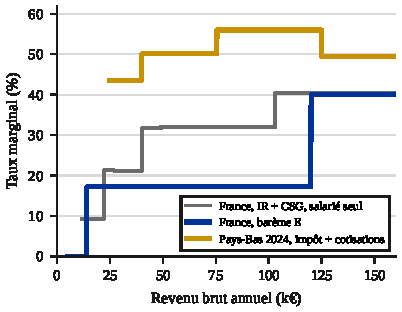
\includegraphics[width=\linewidth]{../figures/nu/ircsg_f11_pays_bas.pdf}
\par{\raggedright\scriptsize\color{encre}Rijksoverheid, Belangrijkste wijzigingen belastingen 2024 ; OpenFisca-France ; calculs de l'auteur.\par Note : Pays-Bas, personne de moins de l'âge de la retraite : tranche à 36,97 \% (dont 27,65 points de cotisations) puis 49,50 \%, plus le retrait du crédit général (6,63 \%) et du crédit d'emploi (6,51 \%). La montée du crédit d'emploi sous 24 812 \euro{} n'est pas représentée. Les assiettes ne sont pas strictement identiques entre les deux pays.
\par}
\vspace{-6pt}
\end{wrapfigure}
\textbf{Pays-Bas.} C'est le précédent le plus proche d'une fusion : les cotisations des assurances nationales (retraite de base, dépendance, survivants) sont prélevées avec l'impôt
sur le revenu, sur la même base et dans les mêmes tranches. En 2024, le barème affiché ne compte que
deux taux : 36,97~\% jusqu'à 75~518~€, dont 27,65~points de cotisations, puis 49,50~\%. La
progressivité passe par deux crédits d'impôt. Le crédit général (3~362~€) se retire au taux de
6,63~\% entre 24~812 et 75~518~€ ; le crédit pour revenus d'activité se retire au taux de 6,51~\%
entre 39~957 et 124~934~€. Le taux marginal réel dépasse donc 50~\% sur une partie de la tranche
inférieure (fiche officielle du gouvernement néerlandais pour 2024). La leçon pour nous : la
progressivité reportée dans des crédits dégressifs rend le barème lisible en façade, mais ses taux
marginaux effectifs le sont beaucoup moins. La franchise du barème E évite ce défaut (figure~\ref{fig:pb}).

\textbf{Royaume-Uni.} La Mirrlees Review (\emph{Tax by Design}, 2011) recommande d'intégrer
impôt sur le revenu et cotisations, dont le lien avec les prestations est devenu presque nul, et
juge qu'un barème optimal peut être approché par « deux ou trois taux et un abattement ».

\textbf{Allemagne et Europe de l'Ouest.} À rendement constant, une flat tax allemande avec
l'abattement existant (26,9~\%) ferait gagner 3,9~\% de revenu disponible au décile le plus aisé
et perdre les déciles 3 à 9 ; avec un abattement relevé à 10~700~€ et un taux de 31,9~\%, le Gini
serait inchangé (Fuest, Peichl et Schaefer, 2008). Paulus et Peichl (2008) trouvent le même
résultat dans dix pays. Le barème E évite ce coût parce qu'il garde deux taux supérieurs.

\textbf{Europe de l'Est.} Les flat taxes de Russie (13~\% en 2001), de Slovaquie (19~\% en 2004)
ou de Roumanie (16~\% en 2005) n'ont produit aucun effet Laffer (Keen, Kim et Varsano, 2008). En
Russie, environ deux tiers de la hausse du revenu déclaré venaient d'un recul de la fraude, et non
d'un supplément d'activité (Gorodnichenko, Martinez-Vazquez et Sabirianova Peter, 2009) : au
sommet, l'élasticité du revenu imposable mesure surtout l'optimisation, et dépend des règles
d'assiette autant que des taux.

\section{Ce qui reste à trancher}

\textbf{L'unité d'imposition.} Le chiffrage applique le barème au foyer fiscal, sans quotient
conjugal ni familial, alors que la CSG est individuelle. Pour un barème presque plat, l'enjeu
diminue beaucoup : entre 14~000 et 120~000~€, un couple paie le même taux marginal qu'il soit
imposé ensemble ou séparément. La question se concentre sur la franchise : une par foyer ou une
par adulte. L'IRCOM ne distingue pas les couples et ne permet pas de chiffrer cette seconde
option ; chaque milliard à compenser demande environ 0,08~point sur le taux unique. Le Conseil des
prélèvements obligatoires (2015) chiffrait à 11,8~Md€ le quotient conjugal transposé dans un impôt
fusionné progressif ; on peut supposer, sans l'avoir vérifié, que ce coût serait bien plus faible
ici. Le traitement des enfants (quotient ou crédit d'impôt
forfaitaire, comme chez Landais, Piketty et Saez, 2011) reste à chiffrer.

\textbf{La contrainte constitutionnelle.} En 2000, le Conseil constitutionnel a censuré une
réduction de CSG pour les bas salaires (décision 2000-437 DC). Il lui reprochait de ne tenir
compte « ni des revenus du contribuable autres que ceux tirés d'une activité, ni des revenus des
autres membres du foyer, ni des personnes à charge ». Un impôt sur l'ensemble des revenus au barème
du foyer, avec une franchise et un traitement des charges de famille, répond à ce motif. Laisser
les revenus au PFU hors barème est à faire expertiser, même si l'IR le fait déjà depuis 2018.

\textbf{L'affectation et les niches.} La CSG finance la Sécurité sociale : une part fixe du nouvel
impôt, environ 62~\% (132 sur 213~Md€), peut lui être affectée. Le chiffrage suppose les
réductions et crédits d'impôt maintenus. Les imputer sur un impôt que tous les foyers paient, et
non plus la moitié d'entre eux, en élargirait le coût.

\textbf{Le résultat au sommet.} Si les revenus au PFU sont logés aussi haut que possible, le
barème E manque la dominance de Lorenz de 1~pour mille entre 100~000 et 300~000~€. Seule une
microsimulation sur fichiers individuels (TAXIPP, INES, OpenFisca) peut trancher ce point et celui
de l'unité d'imposition.

\appendix
\section*{Annexe. Vérifications}

\begin{table}[htbp]\centering\scriptsize
\begin{tabularx}{\linewidth}{@{}>{\raggedright\arraybackslash}p{3.2cm}>{\raggedright\arraybackslash}X>{\raggedright\arraybackslash}p{4.1cm}@{}}
\toprule
Ce qui est testé & Source de comparaison & Résultat \\
\midrule
Composition de la rubrique « salaires » de l'IRCOM & Totaux des cases 2042, revenus 2024 (DGFiP) & 925 Md€ par les cases contre 930 dans l'IRCOM ; pensions 391 contre 393 \\
CSG sur les salaires & Commission des comptes de la Sécurité sociale, mai 2026 (2024 : privé 72,2, public 19,8~Md€) & 91,5 reconstitués contre 92,0 \\
CSG sur les pensions & Même source (retraites 24,8~Md€, invalidité) & Calage du nombre moyen de parts : 1,45 \\
Pensions brutes & Eurostat, pensions de vieillesse, survie, invalidité (412~Md€ en 2023) & 406~Md€ reconstitués pour 2024 \\
Salaires bruts & Eurostat, salaires bruts reçus par les ménages (1~137~Md€) & 1~012~Md€ : l'écart correspond aux non-déclarants et aux salaires de source étrangère, exclus \\
Passage net imposable → brut & OpenFisca-France, cas-types 21 à 250~k€ & Salaires 1,21-1,22 ; CSG 9,04~\% du brut ; pensions 1,04-1,06 (la v1 retenait 1,075) \\
Taux marginaux actuels & OpenFisca, six profils de foyers & La pente entre tranches de la v1 sous-estimait de 10 à 20 points au-dessus de 200~k€ de RFR : corrigé \\
Périmètre & Cases 2042 (PFU environ 90~Md€ ; foncier 38 ; indépendants 80) & La v1 imputait 12,8~\% d'IR au foncier et aux indépendants : corrigé \\
Répartition du PFU entre tranches & Trois hypothèses & Taux unique de E entre 16,6 et 17,7~\% ; dominance de Lorenz dans 3 cas sur 4 \\
\bottomrule
\end{tabularx}
\end{table}


\vspace{6pt}
{\scriptsize\textbf{Références.} Adam et Loutzenhiser (2007), IFS WP 07/21. Atkinson (1970), \emph{JET}
2. Bourguignon et Spadaro (2012), \emph{J. Econ. Inequality} 10(1) (lu : EUROMOD EM9/08). Cabannes, Houdré
et Landais (2014), \emph{Économie et Statistique} 467-468. CCSS (mai 2026), fiche 1.3. Conseil
constitutionnel, décision 2000-437 DC. CPO (2015), \emph{Impôt sur le revenu, CSG : quelles réformes ?}
Fuest, Peichl et Schaefer (2008), \emph{ITAX} (lu : IZA DP 3142). Gorodnichenko, Martinez-Vazquez et
Sabirianova Peter (2009), \emph{JPE} (lu : NBER WP 13719). Hendren (2020), \emph{JPubE} (lu : NBER WP 20351).
Jacobs, Jongen et Zoutman (2017), \emph{JPubE} (lu : Tinbergen DP 16-032). Keen, Kim et Varsano (2008),
\emph{ITAX} (lu : IMF WP 06/218). Kleven et Schultz (2014), \emph{AEJ: Policy} 6(4). Landais, Piketty et
Saez (2011), \emph{Pour une révolution fiscale}. Lockwood et Weinzierl (2016), \emph{JME} 77 (lu : NBER WP
21927). Mirrlees et al. (2011), \emph{Tax by Design}. Paulus et Peichl (2008), EUROMOD EM2/08. Piketty et
Saez (2013), \emph{Handbook of Public Economics} 5. Rijksoverheid (2023), \emph{Belangrijkste wijzigingen
belastingen 2024}. Saez (2001), \emph{REStud} 68. Sicsic (2022), \emph{Fiscal Studies}.\par}

\end{document}
